\documentclass[a4paper, 11pt]{article} % Font size (can be 10pt, 11pt or 12pt) and paper size (remove a4paper for US letter paper)

\usepackage[protrusion=true,expansion=true]{microtype} % Better typography
\usepackage{graphicx} % Required for including pictures
\usepackage{wrapfig} % Allows in-line images

\usepackage{mathpazo} % Use the Palatino font
\usepackage[T1]{fontenc} % Required for accented characters
\linespread{1.05} % Change line spacing here, Palatino benefits from a slight increase by default

\makeatletter
\renewcommand\@biblabel[1]{\textbf{#1.}} % Change the square brackets for each bibliography item from '[1]' to '1.'
\renewcommand{\@listI}{\itemsep=0pt} % Reduce the space between items in the itemize and enumerate environments and the bibliography

\renewcommand{\maketitle}{ % Customize the title - do not edit title and author name here, see the TITLE block below
\begin{flushleft} % Right align
{\LARGE\@title} % Increase the font size of the title

\vspace{30pt} % Some vertical space between the title and author name

{\large\@author} % Author name
\\\@date % Date

\vspace{30pt} % Some vertical space between the author block and abstract
\end{flushleft}
}

%----------------------------------------------------------------------------------------
%	TITLE
%----------------------------------------------------------------------------------------

\title{\textbf{WACC Language Compiler} \\ Project Report} % Title

\author{\textsc{James Lane, Frederick Lindsey, James Long, James Prince} % Author
\\{\textit{Imperial College London}}} % Institution

\date{\today} % Date

%----------------------------------------------------------------------------------------

\begin{document}

\maketitle % Print the title section

%----------------------------------------------------------------------------------------
%	ABSTRACT AND KEYWORDS
%----------------------------------------------------------------------------------------

%\renewcommand{\abstractname}{Summary} % Uncomment to change the name of the abstract to something else

\begin{abstract}
Here we present our project report for the WACC Compiler Lab in the Autumn term of second year for the Computing BEng/MEng. We detail our end product, what our process was during both the design and implementation stages, certain design decisions we made from the start and how we have extended our compiler to go beyond the specification.
\end{abstract}

%\hspace*{3,6mm}\textit{Keywords:} lorem , ipsum , dolor , sit amet , lectus % Keywords

\vspace{20pt} % Some vertical space between the abstract and first section

%----------------------------------------------------------------------------------------
%	ESSAY BODY
%----------------------------------------------------------------------------------------

\section*{Introduction}

We were given the task of designing and implementing a compiler for the WACC language. WACC is a while-like language which is similar in style to many toy languages used in many program verification courses. It has a similar feel to C on a per line basis (i.e. int x = 5;) but also borrows from Haskell in terms of syntax (i.e. fst, snd functions) and ideas (ie. pairs). We were free to choose the language to make the compiler in, though we were strongly encouraged to do it in Java due to the availability of ANTLR and lab support.

%------------------------------------------------

\section*{Product}

%An analysis and critical evaluation of the quality of the WACC compiler you have built. You should consider both whether it meets the functional specification and whether you judge that it forms a sound basis for future development. You may wish to address performance issues.

Our compiler was built in three stages (milestones): The front end, the back end and the extensions. In the front end we perform semantic analysis, create a parse tree - which we then traverse using the visitor pattern to create an AST. The back end then takes this AST and produces assembly code which is generated by calling $ generateCode() $ on the root ProgramNode, which then recursively calls $ generateCode() $ on its children. Once this is generated, it is saved to an $ .s $ (assembly) file in the root directory with the same name as the input file. This can then be passed into a compiler to convert this assembly code into machine code (for example, arm-linux-gnueabi-gcc). \\
However, should the user require the file to be compiled to a specific location, they can call $ ./compile < input > < output > $, saving the output file to the location specified, should this be possible.


We implemented our compiler in Java. There were a few candidate choices for the language: C++ was also a contender, yet in the end we decided Java has richer containers (which we have used throughout), and we wouldn't have to do battle with C++ memory management. Furthermore, with the lab support offered by the department and the use of ANTLR we felt that our speed of development would be much quicker in Java than in C/C++. 

Our front end parses a .wacc file by performing lexical analysis to tokenise the input, we then perform syntactic analysis - throwing an error if the program file is badly formed. We used ANTLR to generate our parser, though we didn't feel the parse tree was compacted enough to perform code generation. Therefore we decided to create our own hierarchy of nodes and created an AST using a visitor derived from the one generated by ANTLR. 
In our hierarchy of nodes, we used an abstract class named ASTNode with an abstract method for checking whether the node was semantically valid - $ isSemanticallyValid() $ which all of the other nodes implemented.  We constructed a tree with a $ ProgramNode $ as the root, and then called $ isSemanticallyValid() $ on it's child nodes. Essentially we propagated the semantic validity check down the tree, checking that each part of the program that a given node represented was semantically valid.

Although we only passed 108/268 test cases at the time we submitted the front end, we managed to increase the number of test cases passed to 267/268 by the time we did our code review. Despite this, we believe our front end to now be functionally correct. 

The backend uses the AST structure we made to semantically check the front end. We added a method that each node implemented - $ generateCode() $ - which generated assembly code and again used the tree structure in order to delegate this down the tree. We created a set of classes in a different package named $ wacc.backend $ which we used to construct instructions. The $ wacc.backend $ package is a mix of classes and enums, in the $ AssemblyInstr $ class we overrode the $ toString() $ method such that it would produce an assembly instruction. This delegation was useful as it meant to convert an $ InstructionBlock $ to a $ String $ we just needed to iterate through the $ ArrayList $ and call the $ toSrting() $ function on each element.

Despite our hard work we were unable to get many test cases to pass. The main reason for this is that we failed to get IO to work correctly in time for the deadline. This resulted in a lot of test cases that should have passed not passing due to the testing relying on a correct implementation of print.
As a result of this, we only managed to pass 123/267 test cases for submission.

Our extensions to the original specification are discussed below.

\section*{Project Management}

%An analysis of the organisation of your group and your use of project management tools (such as Git). You should describe how your group was structured, how you coordinated your work and detail any tools that helped/hindered your progress. You should also discuss what went well and what you would do differently if you were to do the lab again.

As for almost every project, we used git as a versioning tool. Though we were given the source files on gitlab, we decided to transfer this repository over to GitHub so we could make use of some of GitHub's richer external integration features. We initially used Facebook Messenger for communication but we soon switched over to Slack as we were able to split up discussions about different parts of the project into different channels and as a standalone app we found it less distracting than the web interface of Facebook. Furthermore, Slack became a very useful productivity tool when combined with GitHub and CircleCI - a testing and deployment framework. We set up Slack to have discussion channels (\#front-end, \#back-end, \#extensions, \#general) as well as integrated it with GitHub (\#github) and CircleCI (\#testing). Each time we committed on any branch, the code was automatically tested and the result of the test pushed to the \#testing channel. Having this feature meant we had a greater sense of accountability over one's code, as everyone in the group would be notified if the build failed for a particular commit.

Frederick set up the interaction between GitHub, Slack and CircleCI as he had previous experience using this system. \\
It was fundamental as a group to ensure we followed a system of working separately on different components before merging them into the $ master $ branch resembling our tested and working codebase. As part of this process, we all agreed to ensure we used tools such as $ git rebase $ and $ git branch $ to achieve this, maintaining the history of the codebase. \\

Where possible, we also chose to test our code using $ JUnit $, to allow us to identify the side effects of edits. Thankfully, for the most part, our edits did not cause significant failures of tests, largely due to the module structure we employed as discussed above. \\

On reflection, our time management as a group could have been improved. At times it was a struggle to complete various parts, which, had the complexity of certain components been recognised earlier on, could have been avoided.

\section*{Design Choices}

%An analysis of the design choices that you made during the WACC lab.You should discuss the design patterns you used when designing your code and why you chose to use them.

%Why we made our own hierarchy

After looking at the parse tree produced by ANTLR we noticed there were a number of "verticals" which whilst necessary for the correct parsing of the files, created issues when we came to traverse the tree using the visitor pattern. To remedy this we decided to create our own AST hierarchy which we believed would make code generation much easier. When we traversed the parse tree using the visitor pattern we populated our own AST, which was created using different Node classes. The Visitor pattern generated by ANTLR allowed us to create a minified AST, removing the unneeded nodes generated by ANTLR, giving us a compact AST. This was especially useful in the backend, as it allowed us to add our assembly code generation to the AST without having to modify the front end code at all. Thus, we simply performed a single walk of the ANTLR parse tree to form our AST, then a walk of the AST for semantic analysis, and one more walk if the program passes all checks for code generation. \\

One of our most important design choices was to treat each node in our tree as independent. Each node had the responsibility of verifying it's own syntactic and semantic validity, and that of it's children. This design pattern also ensured that the code we wrote would not repeat itself more than necessary, and indeed it meant that testing was far easier to complete. \\

Testing was done using JUnit, with an individual test for each semantic analysis method in every AST node, ensuring that all of our checks were working as intended, and integrating with our Circle CI checks to confirm that submitted changes did not break any previously working functionality. \\

Clearly, due to the way that a program is inherently linked and used as one, this was not entirely possible. The scoping of variables used within each partial of the program had to be considered, and indeed verified. This leads us to our next design choice. \\

We chose to understand and implement the stack/heap that would be in use by the program as a table. This table would hold children that represented scopes below it that would not be seen by the program at it's current level, as well as be referenced by parents who would determine the availability of variables in higher scopes. We then passed this 'symbol' table in our nodes held in the AST. By doing this, each node could access information at it's level and the levels above, giving it the ability to verify its validity using 'knowledge' of where it is in the program. \\

%------------------------------------------------

\section*{Extensions}

%An evaluation of your extensions to your WACC compiler. Youshould describe all of the language extensions, optimisations or other aspects that you have added to your compiler, including how these features can be accessed or viewed. You should also briefly discuss what future extensions you would like to add to your WACC compiler if you had more time.

\subsection*{If without an else}
Our first extension consists of a change to the standard $ IF $ statement included in the WACC language. As per the spec, the standard $ IF $ statement must have an $ else $ branch. However in practice, this might not always be needed. Although we can just have a $ Skip $ statement in the else branch to simulate not having one, this creates less readable code and removing the need for an else branch increases readability of code.

%subtitle: Side effecting assigns (+=, -=, etc)

%subtitle: Side effecting commands (++, --)

%subtitle: Constant string concatenation

\subsection*{A GUI for the compiler}

Finally, we found that when we were learning the $ WACC $ language, something very important was to use the language to understand how it worked. There is no easier way to do this than compile the language into assembly code. It is at this point that the compiler is able to determine syntax errors, or semantic errors and report these back to the user. \\

To use the GUI interface to the compiler that we built, the user runs the following command: \\

\begin{math}
\texttt{./compile -gui}
\end{math} \\

A window will load that allows the user to enter code that follows the WACC language specification. When ready, the user can click the compile button and see the output, should it be available, or errors that prevented output, should it not be available. \\

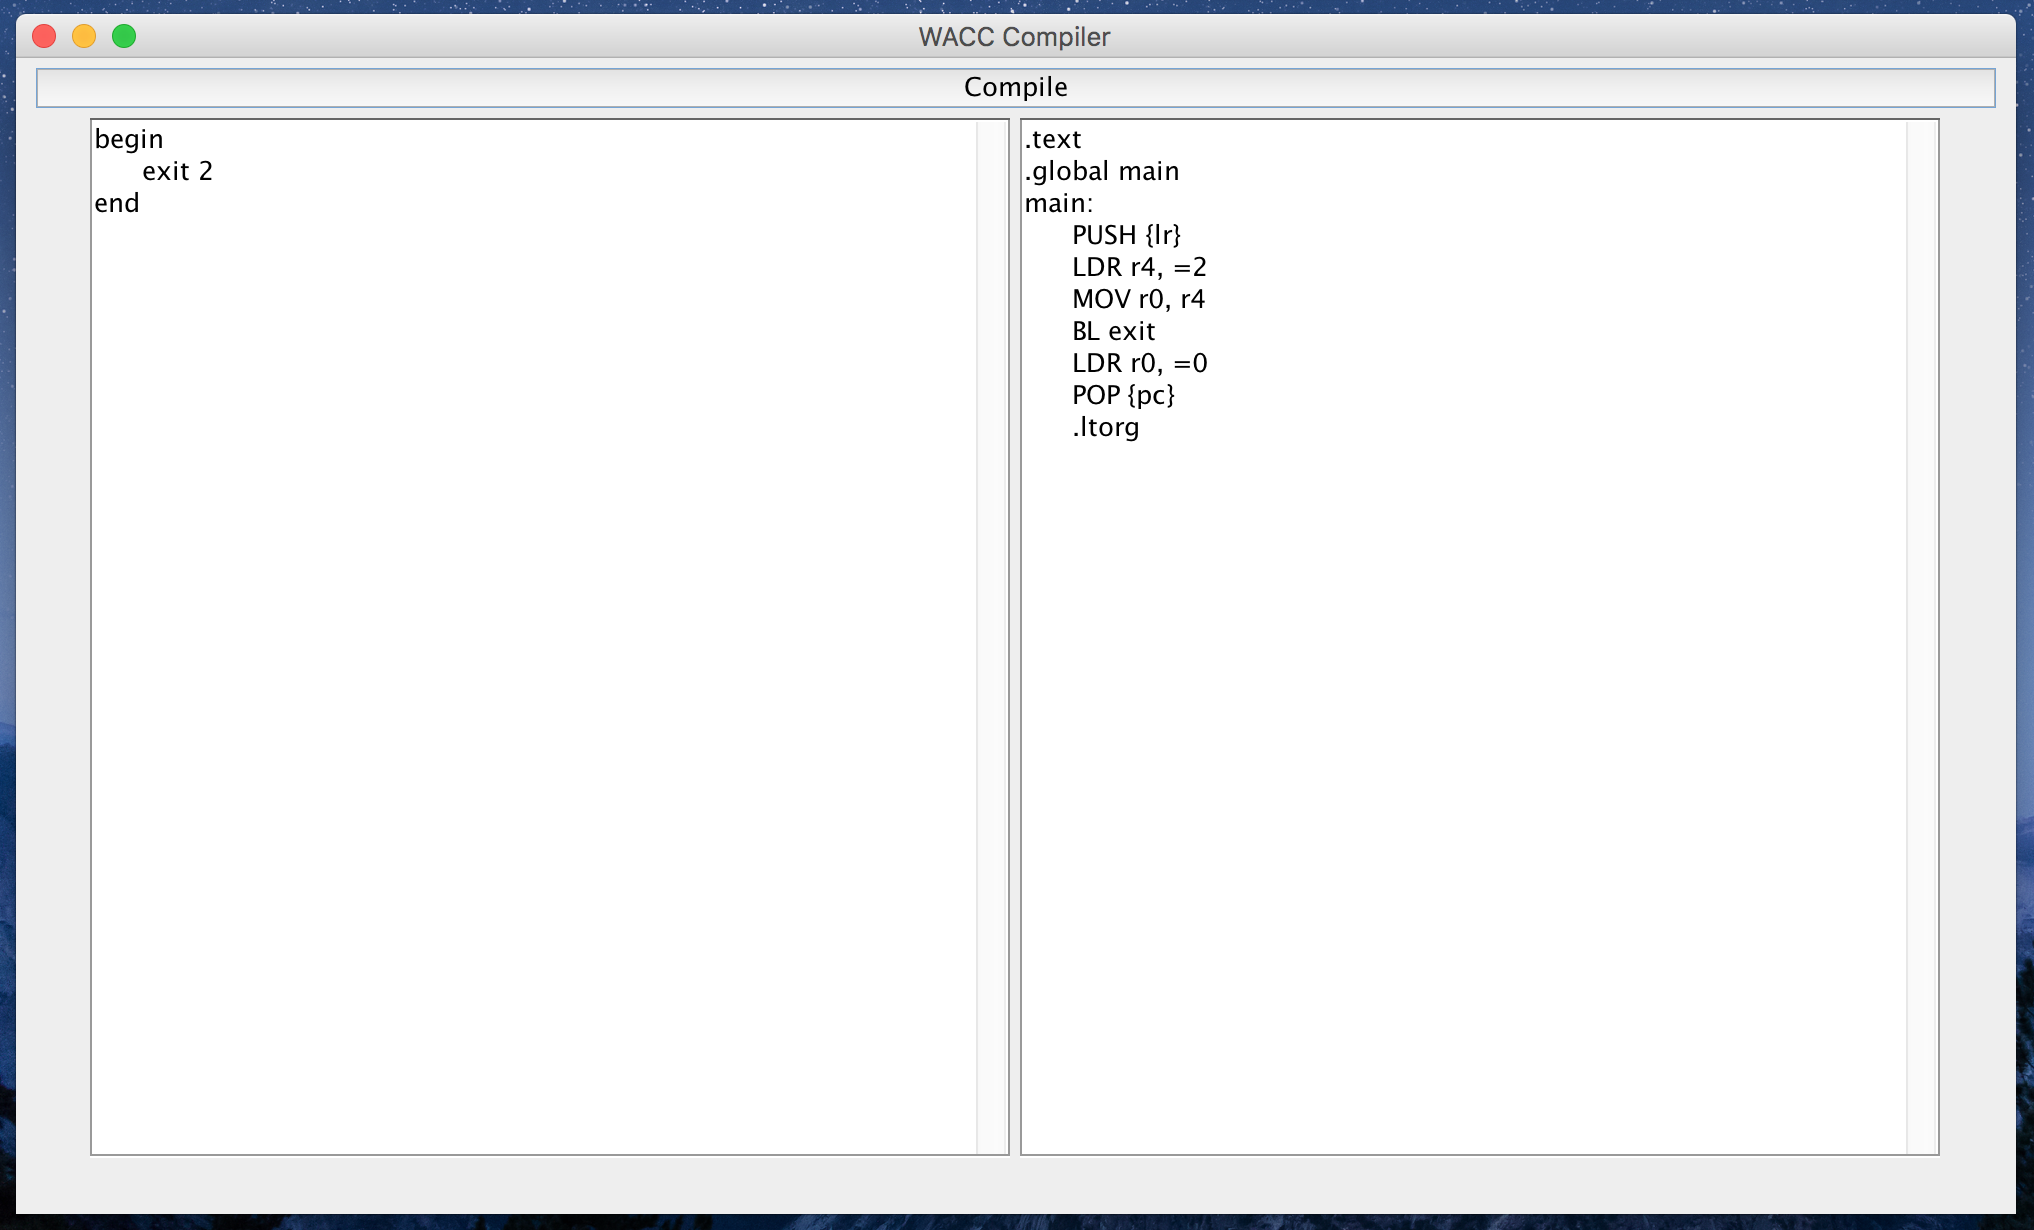
\includegraphics[scale=0.32]{sample-exit2.png} \\

The GUI features an input box on the left, and an uneditable text box on the right which produces output. In the event of errors, the user is presented with a screen similar to below. \\

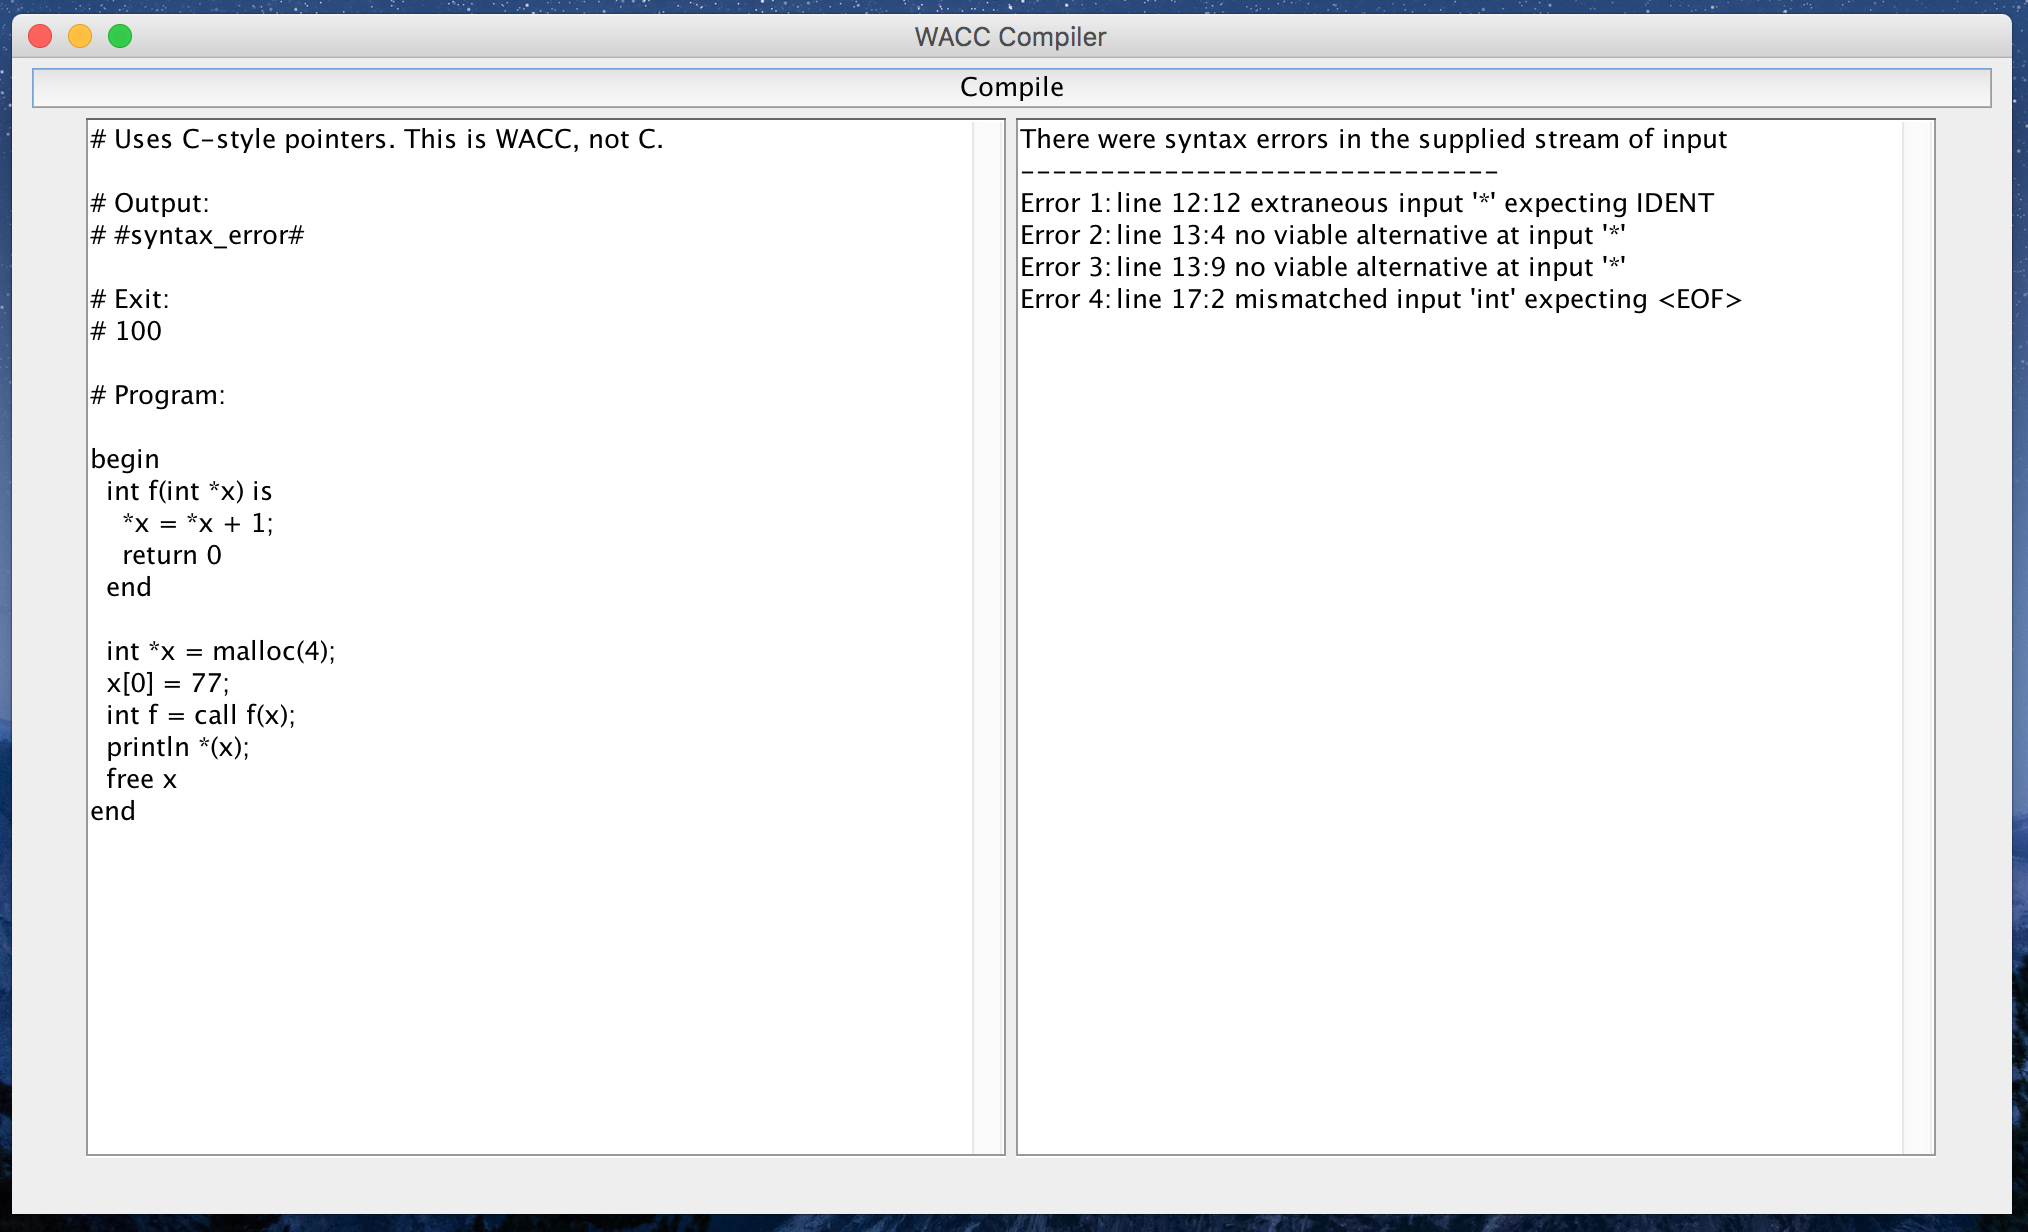
\includegraphics[scale=0.32]{sample-invalid1.png} \\

The above example shows the case where the user has attempted to use a C-like program and compile it using the WACC compiler. Errors are presented to them. \\

Whilst the output box is not editable, the user is able to copy the output and use it in an assembly file which can be evaluated on their system of choice.

%------------------------------------------------

\end{document}